\subsection{Generierung von elliptischen Galaxien}
\subsubsection{Das Navarro-Frenk-White Profil}

Das Navarro-Frenk-White Profil (NFW-profil) ist ein Profil zur Simulation
von Masseverteilungen in N-Körper-Simulationen. Im Grunde genommen bekommt man durch das Profil die
Wahrscheinlichkeit das ein Stern in einem Abstand \( r \) vom Mittelpunkt der
Galaxie existiert.
Die Funktion die dies bewerkstelligt ist im Allgemeinen wie folgt aufgebaut:

\begin{equation} \label{eq:NFW_profile}
  \rho_{NFW}(r) = \frac{ 1 }{ \sqrt{ 2 \pi } \cdot \sigma } \cdot
  \exp \left( \frac{ -\phi(r) }{ \sigma^{ 2 } } \right)
\end{equation}

\begin{equation*}
  \phi(r) = \frac{ 4\pi \cdot G \cdot f_{0} \cdot R_{s}^3 }{ r } \cdot
  ln{ \left( 1 + \frac{ r }{ R_{s} } \right) }
\end{equation*}

Beispiel Werte:

\begin{tabular}{l l l}
  \( sigma \) & = & 200 \\
  \( f_0 \) & = & 0.1 \\
  \( R_s \) & = & 10000 \\
  \( pi \) & = & 3.141592 \\
  \( e \) & = & 2.718281 \\
  \( G \) & = & 4.302e-3 \\
\end{tabular}

Möchte man herausfinden wie wahrscheinlich es ist das ein Stern generiert wird,
setzt man den Abstand des Sternes vom Mittelpunkt der Galaxie in die Formel
(\ref{eq:NFW_profile}) ein. Möchte man z. B. wissen wie wahrscheinlich es ist,
das ein Stern der die Koordinaten \( (x_{1}, x_{2}, x_{3}) \) besitzt generiert
wird, wird der Abstand zum Mittelpunkt der Galaxie mithilfe des Satzes des
Pythagoras berechnet:

\begin{equation}
  r = \sqrt{ {x_{1}}^2 + {x_{2}}^2 + {x_{2}}^2 }
\end{equation}

In dem Beispiel wird also der Wert \( r \) in das NFW-Profil gegeben:

\begin{equation*}
  \rho_{NFW}(r) = \dots = s
\end{equation*}

Als Lösung erhält man einen Wert der in einem Intervall
\( [~\rho(r_{min})~;~\rho(r_{max})~] \) liegt. Rechnet man \( \rho(r_{min}) \) und
\( \rho(r_{max}) \) aus, ist es möglich den jeweiligen Ergebnissen anhand dieser
Werte eine Wahrscheinlichkeit zwischen \( 0 \) und \( 100\% \) zuzuordnen Sodas
es möglich ist zu entscheiden, ob ein Stern bei \( P(x_1 | x_2 | x_3) \) generiert
werden soll oder nicht.

\begin{figure}
  \centering
  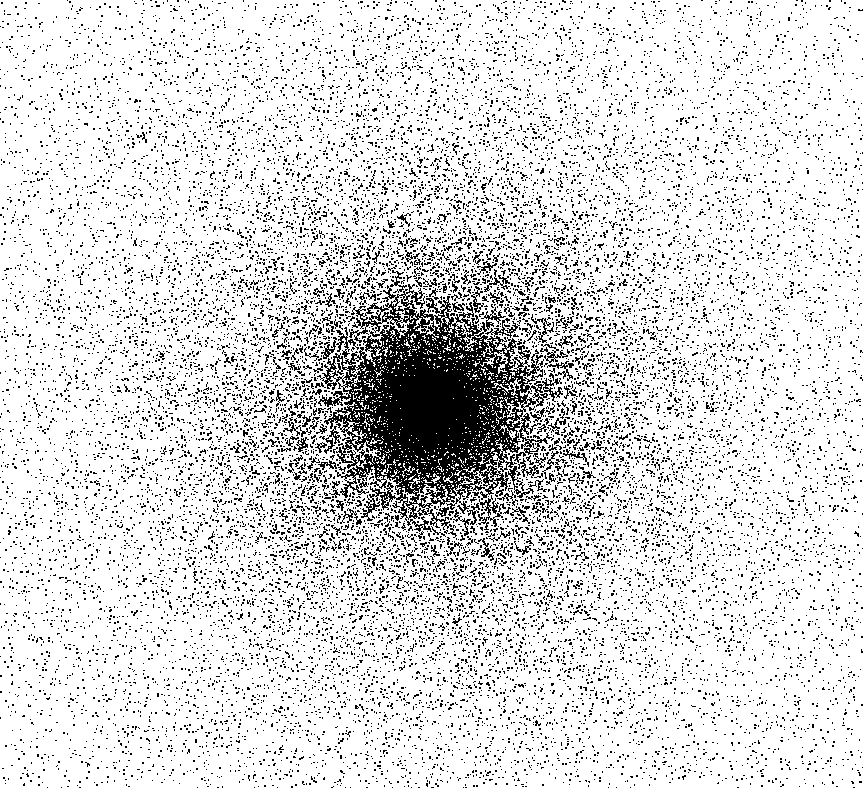
\includegraphics[width=0.75\textwidth]{figs/galaxy}
  \caption{Eine mit dem NFW-profil und der Random Sampling Methode generierte Galaxie}
  \label{fig:galaxy}
\end{figure}

\begin{figure}
  \centering
  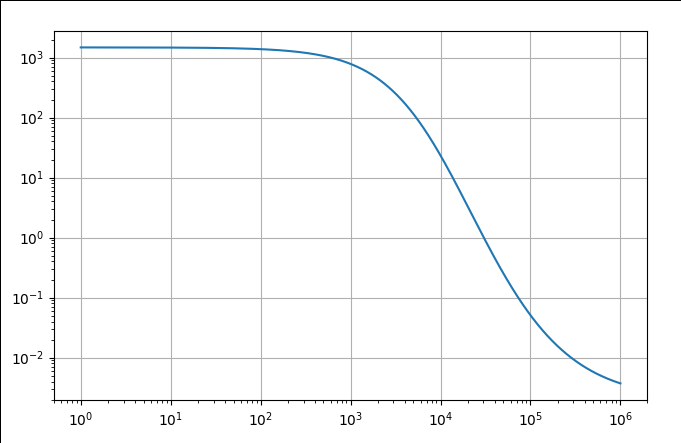
\includegraphics[width=0.75\textwidth]{figs/lookup_table_rho_r_function_grid}
  \caption{
  Die Rho Funktion im Intervall \( [~0~;~10^7 ~] \) geplottet mithilfe von Logarithmischen Achsen. \\
  Die x-Achse beschreibt die Entfernung zum Mittelpunkt der Galaxie \\
  Die y-Achse beschreibt die Warscheinlichkeit das ein Stern generiert wird
  }
  \label{fig:rho}
\end{figure}

\subsubsection{Random Sampling}

Um jetzt herauszufinden ob der Stern bei \( P(x_{1} | x_{2} | x_{3}) \) generiert
wird, wird ein zufälliger Wert \( n \) im Intervall
\( [~\rho(0)~;~\rho(r_{max})~] \) generiert und mit dem Wert \( x \)
verglichen.
Ein Stern wird generiert wenn gilt \( n < x \). Wenn jedoch \( n > x \) gilt
wird kein Stern generiert.
Dieser Prozess wird Random Sampling gennant und ist einer der Knackpunkte wenn
es darum geht die Zeit in der ein Stern generiert wird zu reduzieren. Eine
Möglichkeit dies zu tun sind sogenannten Lookuptabellen (siehe Sektion \ref{subsec:lookup})

\subsubsection{Lookup Tabellen} \label{subsec:lookup}

Um das generieren zu Beschleunigen wird eine sogenannte ``lookuptable''
verwendet. (\( \rightarrow \) \ref{subsec:lookuptable}) dabei wird die Funktion
aus dem NFW-profile (\ref{eq:NFW_profile}) in eine Tabelle geschrieben die im
.csv-format in eine Datei gespeichert. Dies hat den Vorteil das die
Ergebnisse gespeichert vorliegen und somit für andere Berechnungen weiterverwendet
werden können und bei der Berechnung in den Arbeitsspeicher geschrieben werden,
wodurch die Ergebnisse aus der Funkion bei Bedarf vorliegen und nicht erst
berechnet werden müssen.

\subsection{Generierung eines Dunkle-Materie Halos durch Anpassung des NFW-Profils}

Die Rotationskurve von Spiralgalaxien verhält sich in der Realität anders als
in einer Simulation. Der Unterschied lässt sich durch eine Kraft erklären
die Auswirkungen auf Materie haben kann, jedoch nicht sichtbar ist. Dadurch
kann diese Kraft nur durch Rückschlüsse beschrieben werden. Verhält sich ein
Objekt also nicht so, wie es aufgrund der sichtbaren auf es einwirkenden Kräfte
tun sollte, so muss eine andere Kraft vorhanden sein, die das Objekt beeinflussen.
Diese ``Kraft'' entsteht voraussichtlich aufgrund von dunkler Materie.
Dadurch das man Dunkle Materie durch beobachten von Sternen orten kann
indem man berechnet wie sich die Sterne theoretische verhalten sollten und dies mit den
realen Gegebenheiten vergleicht kann man die Funktion die eigentlich die Dichte der
Sternenverteilung (NFW-profil) erklären soll so anpassen das man die Dichte der
Verteilung von dunkler Materie berechnen kann.
Das NFW-profil (\ref{eq:NFW_profile}) kann also so angepasst werden, dass es
statt die Wahrscheinlichkeit das ein Stern generiert wird die Wahrscheinlichkeit
das Dunkle Materie an einem zufälligem Ort existiert, umgebaut werden.
Das NFW-profil (\ref{eq:NFW_profile}) wird also zu (\ref{eq:dark_matter})
umgebaut.

\bigskip

\begin{equation}\label{eq:dark_matter}
  \rho_{NFWDM}(r) = \frac{1}{\sqrt{2 \cdot \pi} \cdot \sigma} \cdot
  e^{\left( - \frac{(\Phi(r)}{\sigma^{2}} \right)}
\end{equation}

\begin{equation}
  \Phi(r) = 1-\frac{1}{(2 \cdot \sigma^{2} )} \cdot
  ( M_{xx} \cdot x^{2} + 2 \cdot M_{xy} \cdot xy + M_{yy} \cdot y^{2} ))
\end{equation}

\bigskip

Eine Mögliche Implementation in der Programiersprache Python als Funktion:

\begin{lstlisting}
def rho(x, y, z):
  a = (1 - ((1) / (2 * (sigma ** 2)))
  b = ( Mxx * x**2 + 2 * Mxy * x * y + Myy * y**2 ) )
  c = a * b
  return rho(x, y, z) * c

def phi(x):
  if x == 0:
    return -4 * pi * f_0 * G * R_s**2

  a = - ( 4 * pi * G * f_0 * R_s ** 3 ) / x
  b = np.log(1. + (x / R_s) )
  c = a * b
  return c
\end{lstlisting}

\subsection{Stauchung und Streckung der Galaxie}

Wird eine Galaxie gestreckt oder gestaucht kann das an der umliegenden Dunklen
Materie liegen. Um solch eine Streckung darzustellen wird wie folgt vorgegangen:
Die Position eines Sternes an einer Achse muss mit einem Skalar multipliziert
bzw. dividiert werden.
Dies ist relativ einfach machbar da die Koordinaten der jeweiligen Sterne
in einer Datei nach dem Format \( x, y, z \) gespeichert sind.
Um die Galaxie vertikal zu strecken wird z. B. für jeden Stern die z-Koordinate
mit dem skalar \( s \) multipliziert. Wenn gestaucht werden soll liegt dieser
Wert im Intervall \( 0 < s < 1 \). Die neue Koordinate für einen Stern ist also
\( x, y, z \cdot s \). Möchte man die Galaxie strecken muss das Skalar \( s \)
im Intervall \( 1 < s < \infty \) liegen.

Indem man ganz grob feststellt in welchen Bereichen der Galaxie der Anteil an
dunkler Materie höher ist kann man dies mit in die Berechnungen einfließen lassen.
In meinem Fall habe ich z. B. ausprobiert einen Richtungsvektor \( \vec{r} \)
zu generieren der von einem Stern in die Richtung der dunklen Materie zeigt.
anschließend hab ich den Richtungsvektor mit einem Skalar \( s \) multipliziert
um die Stärke mit der die Dunkle Energie auf einen jeweiligen Stern wirkt
kontrollieren zu können. Als letztes habe ich dann den Richtungsvektor
mit mit den Koordinaten des Sternes multipliziert um eine theoretische neue
Position für den Stern zu generieren. Tut man dies für alle Sterne entstehen
kleinere sogenannte ''cluster'' in denen sich die Sterne bündeln. Ein Problem
hierbei war, dass es unglaublich rechenaufwendig ist dies für mehrere hunderte
von Tausenden Sternen zu berechnen (siehe Sektion \ref{subsec:big_o}
und \ref{subsec:speeding_things_up})

\subsection{Rechenaufwand} \label{subsec:big_o}

Um den Rechenaufwand in der Informatik darzustellen wird die sogenannte
''O notation'' verwendet. Diese Notation wird verwendet um zu beschreiben
wie viele schritte gebraucht werden um an ein Ziel zu kommen, abhängig von der
Anzahl der ''Objekte'':

\begin{equation}
  O(n) = |\dots|
\end{equation}

Beispiel:

\begin{equation*}
  O(n) = |n^2|
\end{equation*}

Möchte man z. B. die Kräfte zwischen \( n = 100 \) Sternen
berechnen werden \( O(100) = 100^2 = 10000 \) Rechnungen ausgeführt.

Bei einer ''O notation'' von \( n^2 \) bei der Berechnung von
Kräften zwischen den Sternen kann also davon ausgegangen werden das desto
mehr Sterne existieren, die Rechenleistung die gebraucht wird um in derselben
Zeit dieselbe Anzahl an Sternen zu generieren Exponentiell für jeden Stern
Steigen wird.

Eines Optimales Ergebnis wäre eine ''Big O notation'' von \( n\log{n} \),
jedoch ist dies zurzeit nicht ganz möglich.

\subsection{Beschleunigung der Generation} \label{subsec:speeding_things_up}

Die Geschwindigkeit mit der die Sterne generiert werden ist ohne irgendeine Art
von Optimierung unglaublich langsam. Die NFW-Funktion (\ref{eq:NFW_profile})
wird für jeden Stern aufs neue vom Computer berechnet was auf mehrere Tausend
Sterne hochgerechnet unglaublich rechenaufwendig ist.
Ein Weiteres Problem ist, dass das Programm von alleine nur einen Kern
verwendet und somit auf eine menge Rechenleistung verzichtet.
Durch Nutzung von mehreren Kernen kann die Zeit
um \( n \) Sterne zu generieren schnell halbiert oder sogar geviertelt werden.

\subsubsection{Lookuptable} \label{subsec:lookuptable}

Eine weitere Möglichkeit für mehrere Berechnungen Zeit zu Sparen ist, den
entsprechenden Wert aus dem NFW-Profil (Formel \ref{eq:NFW_profile}) vorher zu
berechnen und in eine Tabelle zu schreiben.
Dies kann für z. B. \( 2 \cdot 10^8 \) Werte getan werden was zwar eine ca. 6 GB große
Datei erzeugt, diese kann jedoch innerhalb weniger Sekunden eingelesen werden
und somit das "errechnen" eines entsprechenden Wertes praktisch innerhalb von
Bruchteilen einer Sekunde simulieren indem das Ergebnis einfach aus dem
Arbeitsspeicher ausgelesen wird.

\subsubsection{Mehr Rechenleistung!}

Um mehr Sterne in weniger Zeit zu generieren können verschiedene
Aspekte der Software optimiert werden. Um jedoch ohne Optimierung mehr Sterne
zu generieren kann einfach mehr Rechenleistung verwendet werden. Dies ist im
Grunde genommen die einfachste Möglichkeit mehr Sterne in einer relativ kurzen
Zeitspanne zu generieren: Schon die Verwendung von vier statt zwei Kernen
ermöglicht es einem in 30 Min. statt ca. 300 Sterne ca. 600 Sterne zu generieren.

\paragraph{Amazon Web Services} ~\\
Um das Generieren von Galaxien so "profitabel" wie möglich zu machen können
sogenannte ''Amazon Web Services\footnote{
Amazon Web Services (AWS) ist ein US-amerikanischer Cloud-Computing-Anbieter,
der 2006 als Tochterunternehmen des Online-Versandhändlers Amazon.com gegründet
wurde. Zahlreiche populäre Dienste wie beispielsweise Dropbox, Netflix,
Foursquare oder Reddit greifen auf die Dienste von Amazon Web Services zurück.
2013 stufte Gartner AWS als führenden internationalen Anbieter im Cloud
Computing ein.
} ''
(AWS) genutzt werden.
Der Dienst ''EC2'' kostet z.B. mit 60 Kernen und 256GB RAM nur \$3.712 pro Stunde.
Statt mit einem Kern in einer Stunde ca. 600 Sterne zu generieren können
also in einer Stunde 38400 Sterne generiert werden! Möchte man \( 1 \cdot
10 ^ 6 \) Sterne generieren bräuchte man mit einer Geschwindigkeit von
ca. 600 Sternen pro Stunde und 64 Kernen ca. 26 Stunden. Dies kostet umgerechnet
ca. 100\$ (83€).
Eine weitere Möglichkeit besteht darin, Virtuelle Server von Netcup anzumieten.
Hierbei kosten z.B. 6 Kerne für einen Monat 8€ wodurch man frei nach Belieben
den ganzen Tag Galaxien generieren kann.

\subsubsection{Nichts in der Konsole ausgeben}~\\
Ein Vorgang der erstaunlicherweise sehr viel Rechenleistung erfordert, ist
der Vorgang beim Ausgeben von Text in die Konsole. Gibt man jede potentielle
Koordinate in die Konsole aus, stürzt das Programm aufgrund von Zuviel Daten im Arbeitspeicher ab.
Um dies zu umgehen kann z. B. nur jeder 100.000 Wert in die Konsole ausgegeben
werden was jedoch auch überflüssig ist wenn man ungefähr abschätzen kann, wann
das Script fertig gelaufen ist.

\subsection{Nutzung eines neuronalen Netzes zum unbeaufsichtigten generieren von Galaxien}
\subsubsection{Aufbau des neuronalen Netzes}

Ein Neuronales Netz ist wie folgt aufgebaut:

\bigskip

\hrule

\bigskip

\tikzset{%
  every neuron/.style={
    circle,
    draw,
    minimum size=1cm
  },
  neuron missing/.style={
    draw=none,
    scale=2,
    text height=0.333cm,
    execute at begin node=\color{black}$\vdots$
  },
}

\begin{center}
  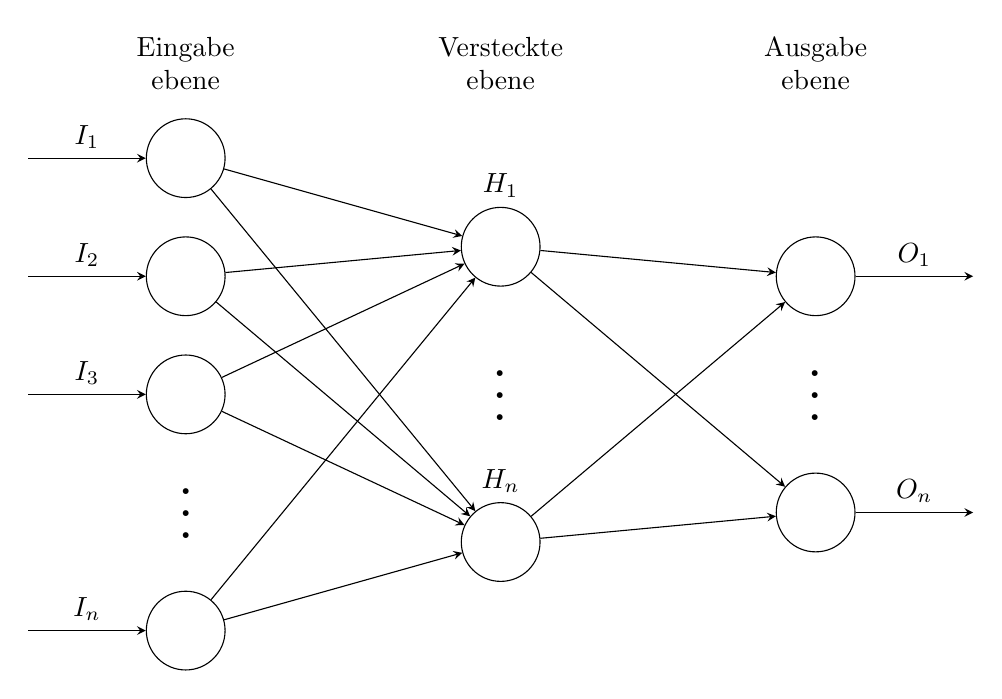
\begin{tikzpicture}[x=2cm, y=1.5cm, >=stealth]

  % Input nodes
  \foreach \m/\l [count=\y] in {1,2,3,missing,4}
    \node [every neuron/.try, neuron \m/.try] (input-\m) at (0,2.5-\y) {};

  % Hidden nodes
  \foreach \m [count=\y] in {1,missing,2}
    \node [every neuron/.try, neuron \m/.try ] (hidden-\m) at (2,2-\y*1.25) {};

  % Output nodes
  \foreach \m [count=\y] in {1,missing,2}
    \node [every neuron/.try, neuron \m/.try ] (output-\m) at (4,1.5-\y) {};

  % Synapses
  \foreach \l [count=\i] in {1,2,3,n}
    \draw [<-] (input-\i) -- ++(-1,0)
      node [above, midway] {$I_\l$};

  \foreach \l [count=\i] in {1,n}
    \node [above] at (hidden-\i.north) {$H_\l$};

  \foreach \l [count=\i] in {1,n}
    \draw [->] (output-\i) -- ++(1,0)
      node [above, midway] {$O_\l$};

  \foreach \i in {1,...,4}
    \foreach \j in {1,...,2}
      \draw [->] (input-\i) -- (hidden-\j);

  \foreach \i in {1,...,2}
    \foreach \j in {1,...,2}
      \draw [->] (hidden-\i) -- (output-\j);

  % Labels
  \foreach \l [count=\x from 0] in {Eingabe, Versteckte, Ausgabe}
    \node [align=center, above] at (\x*2,2) {\l \\ ebene};

  \end{tikzpicture}
\end{center}
\bigskip

\hrule

Im Grunde genommen werden Daten eingespeist und miteinander verrechnet, wodurch
am Ende ein oder mehrere Werte rauskommen mit denen man die verschiedensten
Sachen tun kann. In meinem Fall konnte ich z. B. die durchschnittliche Dichte
von Sternen, die Größe der Galaxie und viele andere Faktoren in das neuronale
Netz einspeisen um am Ende zwei Werte entnehmen. Das neuronale Netz muss
trainiert werden, dabei werden echte funktionierende Daten in das Netz eingespeist
und mit bereits vorhandenen Ergebnissen verglichen. Ist das Ergebnis gut und
stimmt ungefähr mit dem bereits vorhandenen Ergebnis überein wird am Netz selber
nichts getan. Stimmt das Ergebnis aus dem Netz mit dem bereits vorhandenen
jedoch nicht überein, dann werden im neuronalen Netz die sogenannten Synapsen
(Die Verbindungen zwischen den Neuronen (Oben als Kreis dargestellt))
entsprechend anders gewichtet.

\paragraph{Neuronen und Synapsen}

In einem neuronalen Netz sind sogenannte Neuronen (In der Abbildung oben als
Kreis dargestellt) über sogenannte Synapsen (In der Abbildung oben als Linie
zwischen zwei Neuronen dargestellt) miteinander verbunden.
Die Neuronen können als eine Art Funktion gesehen werden. Sie Wandeln die Daten
die sie bekommen mithilfe einer Aktivierungsfunktion in einen Zahlenbereich
zwischen 0 und 1 um. Eine solche Aktivierungsfunktion kann die folgende Form
haben:

\begin{equation}
  S(x) = \frac{1}{1 + e^{-x}}
\end{equation}

Die Synapsen können verschieden gewichtet sein. Bekommt eine Synapse z. B.
einen Eingabewert \( x \), dann kann der Eingabewert mit der Gewichtung \( w \)
der Synapse verrechnet werden um den Ausgabewert \( a \) zu erhalten:

\begin{equation}
  x \cdot w = a
\end{equation}

Für eine weite Ausführung in den Bereich der neuronalen Netze reicht die vorgegebene
Maximalanzahl an Seiten leider nicht, deshalb hier kurz das wesentliche:
Um neuronale Netze effektiv nutzen zu können wird unglaublich viel
Rechenleistung benötigt. Diese habe ich nicht einfach so zur Verfügung, weshalb
ich Kontakt mit verschiedenen Unis und Unternehmen aufgenommen haben um dort
vielleicht Zugang zu einem Hochleistungsrechner zu bekommen. Zum Zeitpunkt der
Abgabe dieser Langfassung (\today) habe ich jedoch noch keine Möglichkeit gehabt
meine Software auf einem solchen Hochleistungs-Rechner laufen zu lassen. Deshalb
habe ich beschlossen die Nutzung von neuronalen Netzen nach hinten zu verschieben,
auch wenn das Thema unglaublich spannend ist.

\bigskip
%
% \paragraph{Was ist ein Neuronales Netz?}
% Ein Neuronales Netz ist ein Gebilde das aus Neuronen und Synapsen besteht.
%
% \paragraph{Was ist ein Neuron?}
% Ein Neuron ist ein Knotenpunkt in einem Neuronalen Netz. Es summiert die
% einkommenden synapsen.
%
% \paragraph{Was ist eine Synapse}
% Eine Synapse ist eine Verbindung zwischen zwei Neuronen. Die Synapsen
% können verschiden gewichtet sein wobei der Eingabewert mit der Gewichtung der
% Synapse multipliziert wird.
%
% \paragraph{Was ist eine Aktivierungsfunktion?}
% Eine Aktivierungsfunktion ist die Funktion die genutzt wird um einen beliebigen
% Wert in einen Wert \( x \) für den gilt \( 0 < x < 1 \).
% Beispiel einer Aktivierungsfunktion:
% Die Funktion (\ref{eq:pyth}) ist der Satz des Pythagoras.
%
% \begin{equation}\label{sigmoid}
%   \frac{1}{1+e^{-x}}
% \end{equation}
%
% \begin{equation}
%   2 + 2 = 4
% \end{equation}
%
% \begin{equation}
%   1 + 1 = 2
% \end{equation}
%
% \begin{equation}\label{eq:pyth}
%   a^2 + b^2 = c^2
% \end{equation}
%
% \paragraph{Was haben die verschiedenen Ebenen zu bedeuten?}
% Die Verschiedenen Ebenen in einem Neuronalen Netzt haben verschiedene
% Funktionen: Die erste Ebene, die sogennante Eingabe Ebene, ist dazu da, eine
% Eingabe in das Netzt einzuschleusen.
% Die Ebenen zwischen der Eingabeebene und er Ausgabeebene werden als Versteckte
% Ebenen bezeichten. Es muss mindestens eine Versteckte Ebene geben damit das
% Netz lernfähig ist, es gibt jedoch keine Begrenzung wieviele Ebenen es geben
% kann.
% Die Ausgabe Ebene ist dazu da die Verarbeiteten Werte auszugeben.
% Hier Bekommt man bei einer Aktivierungsfunktion (\ref{sigmoid}) die eine Ausgabe
% zwischen 0 und 1 liefert einen Wert zwischen 0 und 1.
%
% \paragraph{Was bringen die ``versteckten Ebenen''?}
% Die Versteckten Ebenen liegen zwischen den Ein- und Asugabeebenen. Sie sind
% dazu da das lernen im Neuronalen Netz zu ermöglichen.
%
% \paragraph{Was ist ``Foward Propagation''?}
% Als "Foward Propagation" wird der Vorgang bezwichten, bei dem ein Wert durch
% das Neuronale Netz geschleust wird.
%
% \paragraph{Wie lernt das Neuronale Netz?}
% Das Neuronale Netz lernt indem es immer wieder die Eingabewerte durch das
% Neuronale Netz schiebt. Hierbei werden am Ende die Gewichtugnen der Synapsen
% verändert wodurch das Netz sich immer weiter verändert.
%
% \paragraph{Was ist ``Backward Propagation?''}
% Als "Backward Propagation" wird der Vorgang bezeichnet indem man nachdem man
% einen Wert duch das Netz geschoben hat im Netz zurück geht und mögliche
% Fehlerquellen sucht. Damit kann wenn bereits ein richtiges Ergebniss vorhanden
% ist, wie z.B. bei der Digitalen Bilderkennung eine Zahl, einen Fehlerkoeffizinet
% berechnet werden der dazu genutzt wird ein besseres Ergebniss zu erzielen.
%
%
% Das \textbf{Neuronale Netz} besitze mehrere Ebenen: die \textbf{Eingabe ebene},
% die \textbf{Versteckte Ebene(n)} und die \textbf{Ausgabe Ebene}.
% Diese Ebenen bestehen aus sogennanten \textbf{Neuronen} die wie im Menschlichen
% Gehirn Informationen aufnehmen und weitergeben. Die Eingabe kann verschieden
% gewichtet sein, es kann also sein das eine Eingabe eine Gewichtung von
% \( 10\% \) hat und eine andere eine Gewichtung von \( 90\% \).
% Die Eingabe Ebene ist dazu da eine Eingabe inform einer Matrix an die
% verschiedenen Neuronen in der Versteckten Ebene weiterzuleiten.
% Die Versteckte Ebene verarbeitet die Information aus der Matrix und leitet
% diese an die Ausgabe Ebene weiter die die Information ausgibt.
% \par
% Das sogennante ''Trainieren`` ist der Prozess, bei dem die Gewichtung der
% Neuronen so Verändert wird, damit ein gewünschtes Ergebnis herrauskommt.
% Beispiel: man möchte ein Neuronales Netz darauf Trainieren eine Galaxie zu
% Identifizieren, dann werden ganz viele positiv Beispiele durch das Netz gejagt
% welche die Gewichtung immer weiter anpassen. In der Ausgangs Ebene wird dann
% mithilfe zweier Neuronen entweder dargestellt das das eingegebene Bild eine
% Galaxie ist oder das das eingegebene Bild eben keine Galaxie ist.
%
% \subsubsection{Nutzung eines Neuronalen Netztes zur verbesserung von Galaxien Simulationen}
%
% Möchte man mithilfe eines Neuronalen Netztes vorhandene Galaxiensimulationen
% verbessern, wird wie im folgenden Diagramm zusehen vorgegangen:
%
% \begin{tikzpicture}
% [node distance = 4cm, auto, ->, on grid]
%
% \node [draw, minimum width=3cm, text depth = 1cm] (galaxy) {Galaxie};
% \node [draw, right of=galaxy] (neural_net) {Neuralonales Netz};
%
% \node [draw] (yes) [right of=neural_net] {Ja}
% node [right=3cm of yes, align=center] {Galaxie ist eine Galaxie};
%
% \node [draw] (no) [below=2cm of neural_net] {Nein}
% node [right=3.5cm of no, align=center] {Galaxie ist keine Galaxie \\
% \( \rightarrow \) ändere parameter und \\generiere eine neue Galaxie};
%
%
% \draw[->, line width=0.25mm] (galaxy) -- (neural_net)
% node [above=1cm of neural_net, align=center] {Testet ob die Eingabe \\eine
% Galaxie ist oder nicht};
%
% \node[draw, yshift=5mm] (paramter) at (galaxy.south) {paramter};
%
% \draw[->, line width=0.25mm] (neural_net) -- (yes);
% \draw[->, line width=0.25mm] (neural_net) -- (no);
%
% \path[line width=0.25mm] (no) edge [bend left] node {} (paramter);
%
% \end{tikzpicture}

\subsection{Spiralgalaxien}

Spiralgalaxien sind im allgemeinen faszinierende Gebilde: Aus mehreren Millionen
Sternen entsteht eine Reisige Spirale. Dies zu simulieren ist jedoch unglaublich
Rechenaufwendig weshalb ich dies bisher nur mir kleineren Galaxien durchgeführt
habe. Das Problem ist, dass die Kräfte zwischen jedem Stern und jedem anderem
Stern ausgerechnet werden müssen was wie in Sektion \ref{subsec:big_o} beschrieben
mit steigender Anzahl an Sternen eine Exponentielle Steigerung der Rechenzeit
hervorruft.

\par Ein interessanter Aspekt der Spiralgalaxien den ich in die Simulationen
einzubauen ist die Diskrepanz zwischen der realen Position
der Sterne und der berechneten Position durch die Auf Dunkle Materie geschlossen
wird.

\subsubsection{Das n-Körper Problem}

(nach der Ph.D. Thesis von Jakub Schwarzmeier s. 18 - 22, Pilsen 2007)

Das sogenannte \( N \)-Körper Problem wird dazu genutzt um ein System mit
\( N \)-Körpern zu simulieren. Hierbei müssen alle von außen einwirkenden
Kräfte \(\vec{F_{i}} \) mit eingerechnet werden, im falle von Galaxien also die
universelle Gravitationsregel von Newton.

\begin{equation}
  m_{i} \cdot \frac{d\vec{v_{i}}}{dt} = \vec{F_i}
\end{equation}

Für zwei Punkte in einer Galaxie gilt nach der universellen Gravitationsregel von
Isaac Newton:

\begin{equation}
  m_{i} \cdot \frac{d\vec{v_{i}}}{dt} =
  G \cdot \frac{m_{i} \cdot m_{j}}{r^{3}_{ij}} \cdot \vec{r_{ij}}
\end{equation}

bzw.

\begin{equation}\label{eq:n-body-2nd}
  \frac{d^{2}\vec{r_{i}}}{dt^{2}} =
  G \cdot \sum_{j = 1} \frac{m_j}{r^{3}_ij} \cdot \vec{r_{ij}}
\end{equation}

Die neue Position und Geschwindigkeit eines Körpers wird mithilfe der bereits
bekannten Beschleunigung berechnet, was zu der Formel (\ref{eq:n-body-2nd}), die
eine zweite Ableitung enthält, führt. Die Formel (\ref{eq:n-body-2nd}) kann
jedoch in zwei neue Formeln umgeschrieben werden, die jeweils nur eine erste
Ableitung enthalten:

\begin{align}\label{eq:hamilton}
  \frac{d\vec{r_{i}}}{dt} &= \vec{v_i} \\
  \frac{d\vec{v_{i}}}{dt} &= G \cdot \sum_{j = 1} \frac{m_j}{r^{3}_{ij}}
  \cdot \vec{r_{ij}}
\end{align}

Die Formeln (\ref{eq:hamilton}) entsprechen der Bewegungsgleichung nach
Hamilton. Möchte man nun die Position der einzelnen Sterne berechnen, müssen
die Werte aus der Funktion in für einen Computer darstellbare Werte umgewandelt
werden.

Eines der Probleme um die Bewegung eines Sternes zu formulieren liegt dabei,
einen Anfangswert für die Bewegung zu finden. Dies wird durch die folgende
Formel gelöst:

\begin{equation}
  x_{t + 1} = x_{t} + \Delta t \cdot F(x_{i}, t_{i})
\end{equation}

Die Position eines Sternes nach einer Zeit von \( \Delta t \) wird durch die
vorherige Position und die auf der Stern wirkenden Kräfte bestimmt.
Der Term \( \Delta t \cdot F(x_{i}, t_{i}) \) wird auch als erster Schritt in
der Taylor-reihe bezeichnet mit der weitere Punkte anhand der Ableitung
vorheriger Punkte errechnet werden können.
Die Veränderung der Position kann aus der Formel (\ref{eq:hamilton}) abgeleitet
werden:

\begin{align}
  \Delta \vec{r_{i}} &=
  \vec{v_{i}} \cdot \Delta t \\
  \Delta \vec{v_{i}} &=
  G \cdot \Delta t \cdot \sum_{j = 1} \frac{m_{j}}{r^{3}_{ij}} \vec{r_{ij}}
\end{align}

\subsubsection{Unterteilung des Vektorraumes in verschiedene Zellen}
Die Kräfte die innerhalb der Galaxie wirken können mithilfe eines Vektorraumes
dargestellt werden. Dabei kann jedem Punkt im Raum ein Vektor zugewiesen werden.
Der Vektorraum im falle von Galaxien stellt erstmal nur die Kräfte, die die
Sterne aufeinander auswirken da.
Um nicht unendlich viel rechnen zu müssen wird der Vektorraum in verschiedene
Zellen unterteilt in denen jeweils die mittlere Kraft berechnet wird.

\subsubsection{Berechnung der wirkenden Kräfte}
Die wirkenden Kräfte können wie in Formel (\ref{eq:gravitation_law}) zu sehen
berechnet werden:

\begin{equation}\label{eq:gravitation_law}
  F_{1} = F_{2} = G \cdot \frac{m_{1} \cdot m_{2}}
  {\sqrt{(a_1 - b_1)^2 + (a_2 - b_2)^2 + (a_3 - b_3)^2}}
\end{equation}

\begin{tabular}{l l}
\( F_1 , F_2 \) & Wirkende Kräfte zwischen zwei Massen \\
G & Gravitationskonstante \( 6,67408 \cdot 10^{-11} \frac{m^3}{kg \cdot s^2} \) \\
\( m_1 \) & Erste Masse \\
\( m_2 \) & Zweite Masse \\
\( r \) & Abstand der Massen
\end{tabular}

\paragraph{Masse der Sterne}
Die Masse der Sterne ist einer der entscheidende Faktoren wenn es darum geht
Galaxien zu generieren: verändert man die Masse der Sterne verändert sich sofort
das gesamte Gleichgewicht in der Galaxie was zu unerwarteten Ereignissen führen
kann.
\par Allgemein gesehen werden zwei Variablen gebraucht: die
\textbf{Minimalmasse} und die \textbf{Maximalmasse}. Zwischen diesen beiden
Werten werden zufällig Werte generiert und den Sternen zugewiesen.
\par Die Veränderung der Masse wird erstmal nicht berücksichtigt.

\paragraph{Abstand der Sterne}
Der Abstand der Sterne kann mit dem Satz des Pythagoras (Formel
(\ref{eq:pytagoras})) berechnet werden.

\begin{equation}\label{eq:pytagoras}
  r_{a, b} = \sqrt{(a_x - b_x)^2 + (a_y - b_y)^2 + (a_z - b_z)^2)}
\end{equation}

\subsection{Weiteres}
Um die Simulation zu beschleunigen können andere Simulationsmodelle
verwendet werden wie z. B. die Kräfte in verschiedenen Feldern berechnen um
diese anschließend weiter zu evaluieren.

\begin{figure}
  \centering
  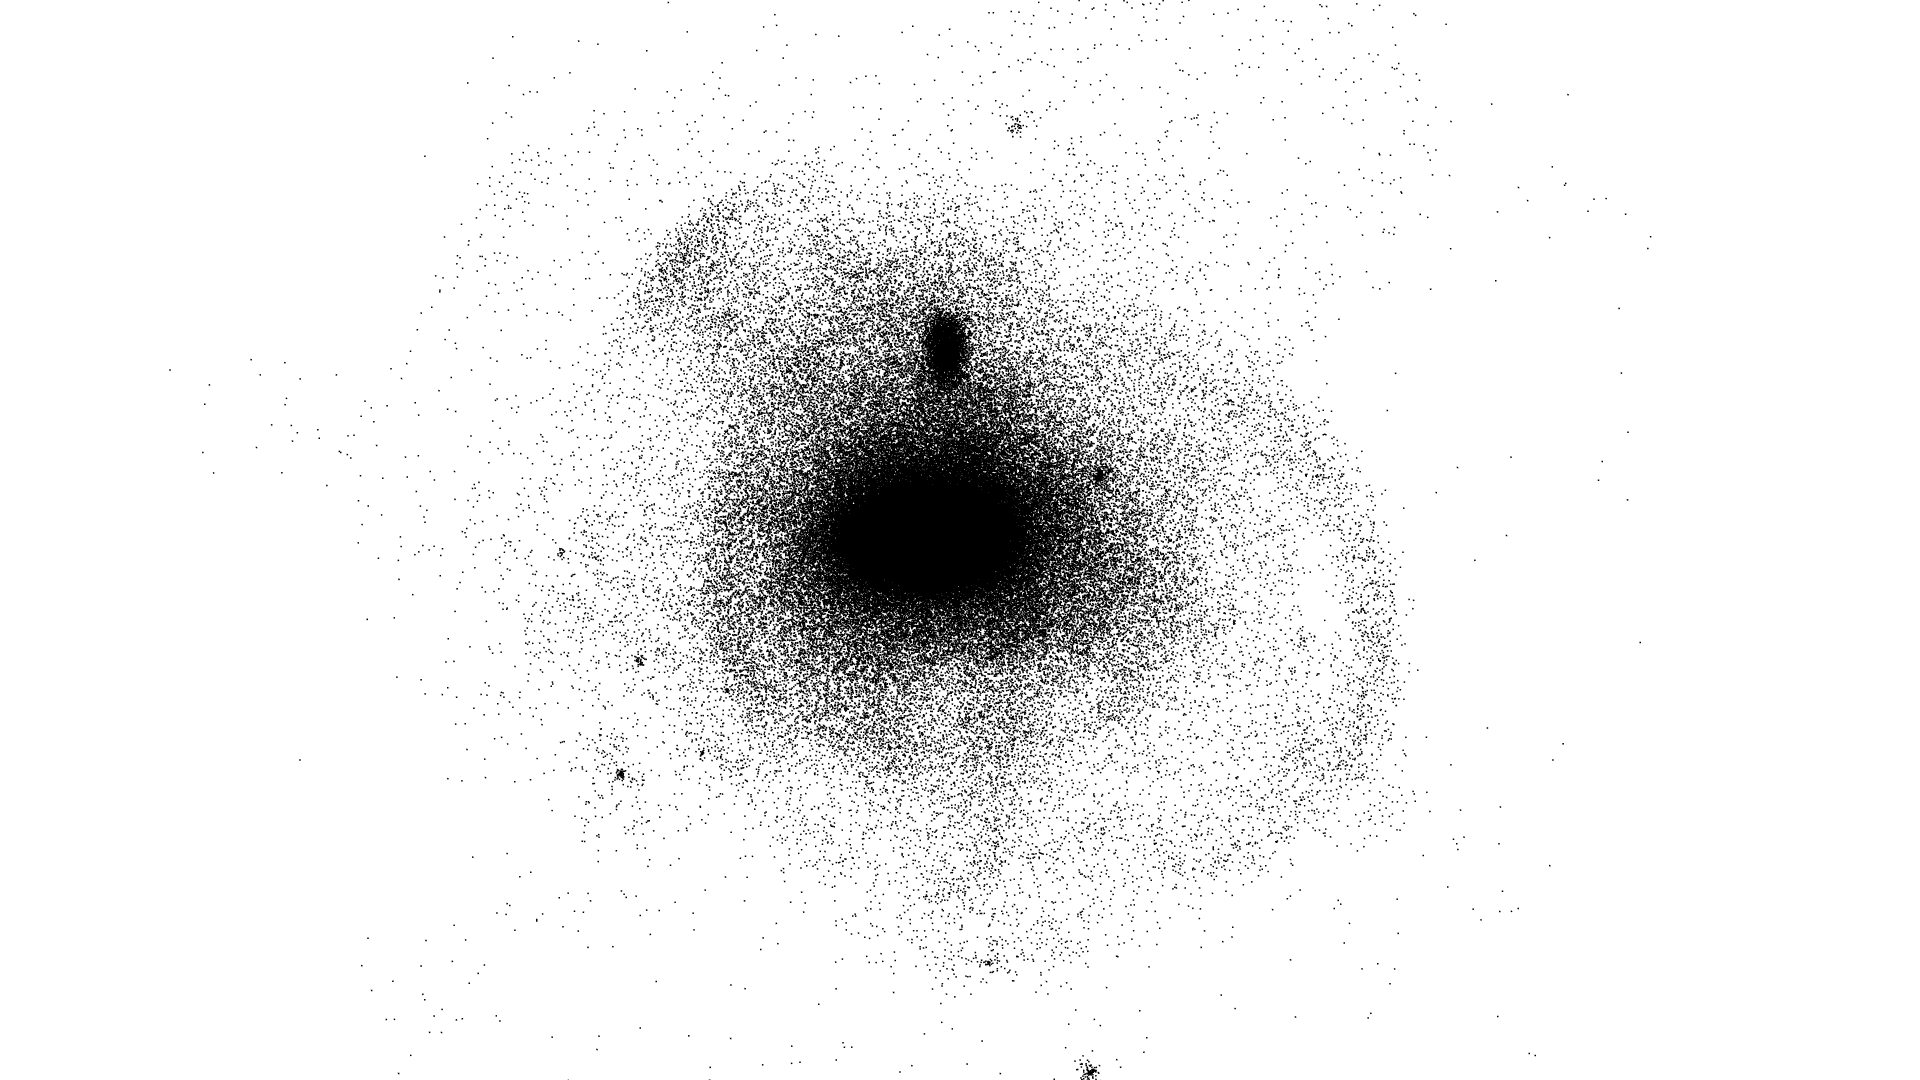
\includegraphics[width=0.75\textwidth]{figs/spiralgalaxy}
  \caption{Eine Spiralgalaxie generiert mithilfe von Daten aus dem Max-Plank-Institut in Heidelberg}
  \label{fig:spiralgalaxy}
\end{figure}
